In this chapter I aim to describe the proposed architecture of the solution, starting with a high-level glance -- the component diagram.

The smartwatch requires an application to propagate the data from the heart rate sensor to the smart phone application.
Once the raw data is received, it is combined with GPS data from the phone and forwarded through the 'biometric and GPS raw data exchange' interface to the IoT platform, where it gets processed and saved.
When the smartphone application requires it, it requests the processed data through the 'processed data retrieval' and displays it.

\begin{figure}[h]
    \tmpframe{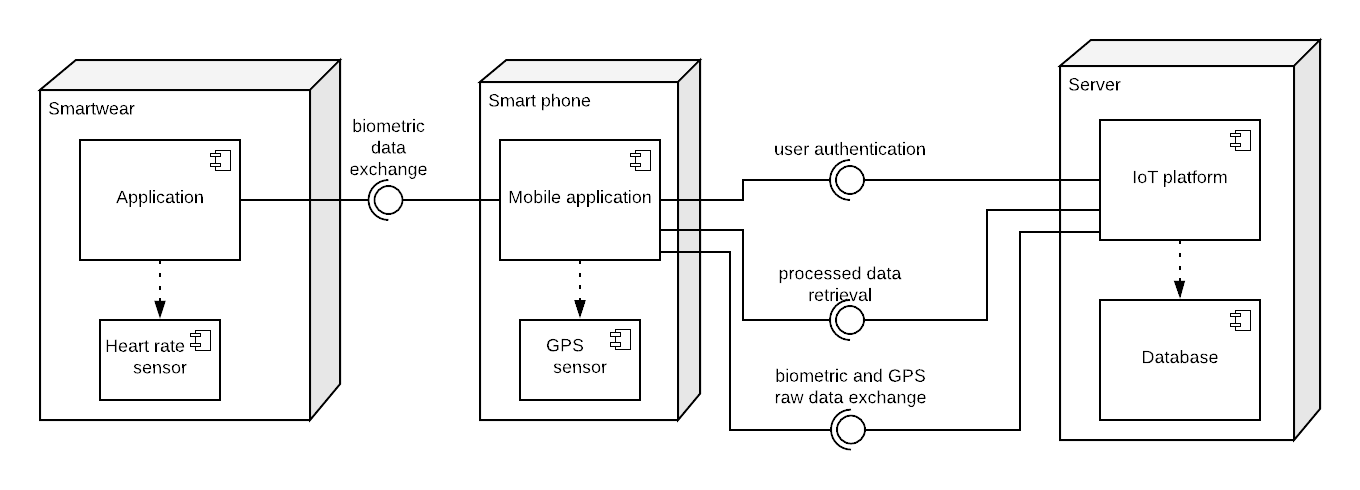
\includegraphics[width=\textwidth]{component.png}}
    \caption{Component diagram of the designed IoT solution}
\end{figure}

Depending on the number and complexity of the features in the future, it is also possible to introduce a web client in order to make the smartphone APP lighter and easier to navigate.

The watch communicates with the phone application over Bluetooth, with the watch application acting as a server, providing information for the client phone application.
The phone application connects to the server using the phone's Internet connection.

